\documentclass[12pt,letterpaper, onecolumn]{exam}
\usepackage{amsmath}
\usepackage{amssymb}
\usepackage{commath}
\usepackage{physics}
\usepackage{multirow}
\usepackage{float}
\usepackage{relsize}
\usepackage{tikz}
\usepackage[lmargin=71pt, tmargin=1.2in]{geometry}  %For centering solution box
\usepackage{clrscode}
\usepackage{listings}
\usepackage{xcolor}
\usepackage{pdfpages}
\usepackage{enumitem}
\definecolor{codegreen}{rgb}{0,0.6,0}
\definecolor{codegray}{rgb}{0.5,0.5,0.5}
\definecolor{codepurple}{rgb}{0.58,0,0.82}
\definecolor{backcolour}{rgb}{0.95,0.95,0.92}
\usetikzlibrary{arrows.meta}
\usetikzlibrary{patterns}
\graphicspath{ {./images/} }

\lstdefinestyle{mystyle}{
    backgroundcolor=\color{backcolour},   
    commentstyle=\color{codegreen},
    keywordstyle=\color{magenta},
    numberstyle=\tiny\color{codegray},
    stringstyle=\color{codepurple},
    basicstyle=\ttfamily\footnotesize,
    breakatwhitespace=false,         
    breaklines=true,                 
    captionpos=b,                    
    keepspaces=true,                 
    numbers=left,                    
    numbersep=1pt,                  
    showspaces=false,                
    showstringspaces=false,
    showtabs=false,                  
    tabsize=2
}

%\lstset{style=mystyle}
\lhead{CAP 5610 Assignment \#2 Solution\\}
\rhead{Arman Sayan\\}
% \chead{\hline} % Un-comment to draw line below header
\thispagestyle{empty}   %For removing header/footer from page 1

\begin{document}

\begingroup  
    \centering
    \LARGE CAP 5610\\
    \LARGE Assignment \#2 Solution\\[0.5em]
    \large \today\\[0.5em]
    \large Arman Sayan\par
\endgroup
\rule{\textwidth}{0.4pt}
\bracketedpoints   %Self-explanatory
\printanswers
\renewcommand{\solutiontitle}{\noindent\textbf{Ans:}\enspace}   %Replace "Ans:" with starting keyword in solution box
\qformat{\large \textbf{\thequestion \quad \thequestiontitle \quad [\thepoints] \hfill}}
\renewcommand{\thepartno}{\arabic{partno}}
\renewcommand{\partlabel}{\thepartno.}

\begin{questions}
    \titledquestion{Types of Attributes}[10]

    Solution for Q1:
    
    %Classify the following attributes as nominal, ordinal, interval, ratio. \textbf{\underline{Explain why}}.

    %\begin{enumerate}[label=(\alph*)]
    %    \item Rating of an Amazon product by a person on a scale of 1 to 5
    %    \item The Internet Speed
    %    \item Number of customers in a store.
    %    \item UCF Student ID
    %    \item Letter grade (A, B, C, D)
    %\end{enumerate}
    
    \begin{solution}
        The classification of the attributes is as follows:

        \begin{enumerate}[label=(\alph*)]
            \item Rating of an Amazon product by a person on a scale of 1 to 5: \textbf{Ordinal}. 
            
            Ratings on a scale have a meaningful order or ranking, but the differences between each rating values are not necessarily equal. 
            For example, the difference between a rating of 1 and 2 may not be the same as the difference between a rating of 4 and 5, but we can sort these ratings from
            5 as the best all the way to the 1 as the worst rating.
            Furthermore, for ordinal attributes like rating, we cannot perform arithmetic operations such as addition or multiplication as they are not meaningful.
            Hence, rating has the distinctness and order properties of ordinal attributes.

            \item The Internet Speed: \textbf{Ratio}. 
            
            The Internet speed has a meaningful difference and a true zero, meaning that ratios also make sense. 
            For instance, 100 Mbps is twice as fast as 50 Mbps, and 0 Mbps means no internet speed.
            Furthermore, we can perform arithmetic operations such as addition and multiplication on internet speed.
            Hence, internet speed has the distinctness, order, and all arithmetic properties of ratio attributes.

            \item Number of customers in a store: \textbf{Ratio}.
            
            The number of customers has a meaningful difference and a true zero, meaning that ratios also make sense.
            To give an example, 100 customers is twice as many as 50 customers, and 0 customers means no customers.
            Furthermore, we can perform arithmetic operations such as addition and multiplication on the number of customers.
            Hence, the number of customers has the distinctness, order, and all arithmetic properties of ratio attributes.

            \item UCF Student ID: \textbf{Nominal}. 
            
            The UCF student ID is a unique identifier or label for each student, but it does not have any meaningful order or ranking.
            To give an instance, a UCF student ID of 1234567 is not better or worse than a student ID of 4567890.
            Furthermore, we cannot perform arithmetic operations such as addition or multiplication on UCF student IDs as they are not meaningful.
            Hence, UCF student ID has the distinctness property of nominal attributes.

            \item Letter grade (A, B, C, D): \textbf{Ordinal}.
            
            Letter grades have a meaningful order or ranking, but the differences between each grade are not necessarily equal.
            To illustrate, the difference between a grade of A (4.0) and B (3.25) may not be the same as the difference between a grade of C (2.50) and D (2.0), but we can
            sort these letters from the best grade to achieve to worst grade to achieve.
            Furthermore, we cannot perform arithmetic operations such as addition or multiplication on letter grades as they are not meaningful.
            Hence, letter grades have the distinctness and order properties of ordinal attributes.
        \end{enumerate}
    \end{solution}

    \pagebreak

    \titledquestion{Distance/Similarity Measures}[20]

    %Given the four boxes shown in the following figure, answer the following questions. In the 
    %diagram, numbers indicate the lengths and widths and you can consider each box to be a vector 
    %of two real numbers, length and width. For example, the top left box would be (2,1), while the 
    %bottom right box would be (3,3). Restrict your choices of similarity/distance measure to 
    %Euclidean distance and correlation. \textbf{\underline{Please explain your choice}}.

    %\begin{figure}[h]
    %    \centering
    %    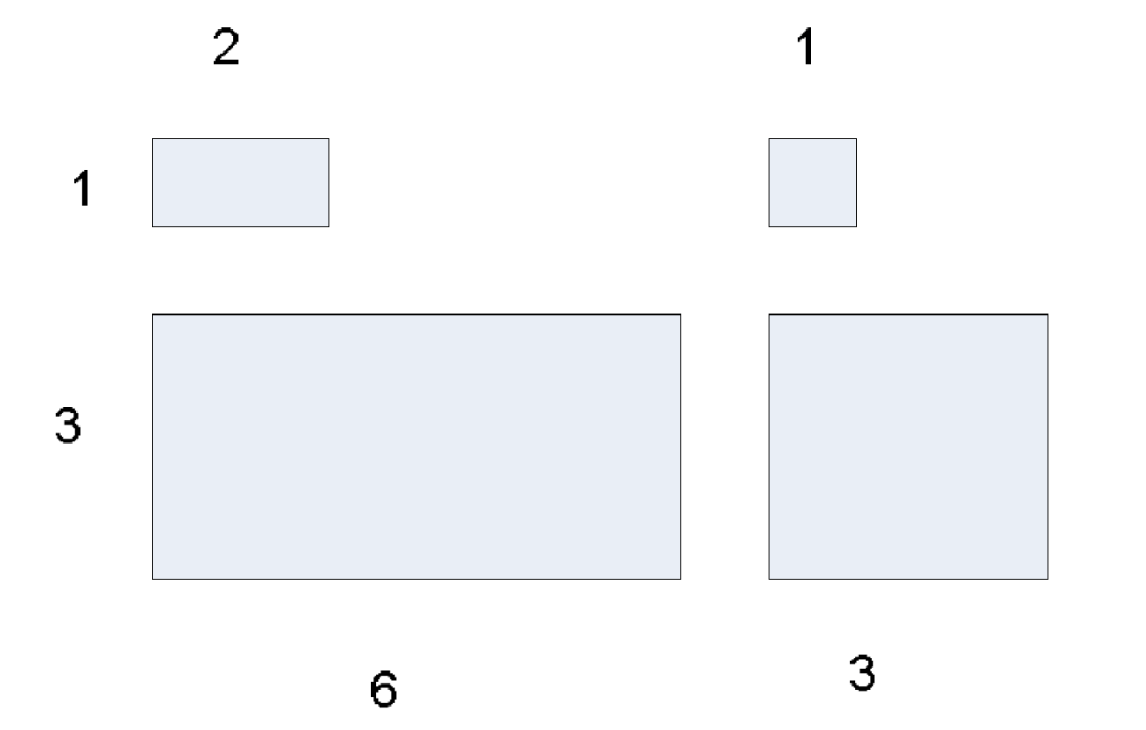
\includegraphics[width=0.65\textwidth]{boxes.png}
    %\end{figure}

    \begin{parts}

        \part[10] Solution for Q2 Part 1:
        %Which proximity measure would you use to group the boxes based on their
        %shapes (length-width ratio)?

        \begin{solution}
            To group the boxes based on their shapes (length-width ratio), the best proximity measure to use is a \textbf{correlation similarity measure} 
            instead of the Euclidean distance. This is because correlation measures the strength and direction of the linear relationship between two variables,
            which in this case are the length and width of the boxes. By using correlation, we can capture the shape of the boxes regardless of their size or position.

            In other words, correlation measures the similarity in the pattern of the length and width values, which is what we are interested in when grouping
            the boxes based on their shapes.

            Since we are interested in shape similarity, the key idea is to check if the length-width ratio of two boxes is consistent.

            For the given 4 boxes, we can calculate the correlation between their length and width values as
            \begin{center}
                $\displaystyle{ratio_{TL} = \frac{2}{1} = 2.0}$

                $\displaystyle{ratio_{TR} = \frac{1}{1} = 1.0}$

                $\displaystyle{ratio_{BL} = \frac{6}{3} = 2.0}$

                $\displaystyle{ratio_{BR} = \frac{3}{3} = 1.0}$
            \end{center}

            By looking at the figure and ratios calculated, we can see that the boxes have different sizes and positions, but their shapes are similar.
            To give an instance, we can see that the top-left box (2,1) has the same ratio as bottom-left box (6,3), making them similar in shape.
            Similarly, the top-right box (1,1) has the same ratio as bottom-right box (3,3), making them similar in shape.

            
            Euclidean distance would not reflect that similarity because it would consider the absolute difference between the length and width values.

        \end{solution}

        \part[10] Solution for Q2 Part 2:
        %Which proximity measure would you use to group the boxes based on their
        %size?

        \begin{solution}
            To group the boxes based on their size, the best proximity measure to use is \textbf{Euclidean distance} instead of correlation similarity measure.
            This is because Euclidean distance measures the absolute difference in both length and width values, which is what we are interested in when grouping
            the boxes based on their overall dimensions.

            In other words, Euclidean distance can be used to group by any size property, which is what we are interested in when grouping
            the boxes based on their size.

            To give an example of grouping by size, we can calculate the Euclidean distance between two boxes $(L_1, W_1)$ and $(L_2, W_2)$, based on their length 
            and width values:

            \begin{center}
                $\displaystyle{d = \sqrt{(L_1 - L_2)^2 + (W_1 - W_2)^2}}$
            \end{center}

            We can apply this formula to the boxes in the figure to group them based on their size. 
            For instance, the Euclidean distance between the top-left box (2,1) and other boxes is:

            \begin{center}
                $\displaystyle{d_{TL,BL} = \sqrt{(2 - 6)^2 + (1 - 3)^2} = \sqrt{20} \approx 4.47}$

                $\displaystyle{d_{TL,TR} = \sqrt{(2 - 1)^2 + (1 - 1)^2} = \sqrt{1} = 1}$

                $\displaystyle{d_{TL,BR} = \sqrt{(2 - 3)^2 + (1 - 3)^2} = \sqrt{5} \approx 2.24}$
            \end{center}

            The lower the Euclidean distance, the more similar the boxes are in size.
            For this reason, we can say that the top-left box (2,1) is more similar in size to the top-right box (1,1) than to the bottom-left box (6,3).

            Correlation similarity measure would not reflect that size similarity because it would consider the pattern of the length and width values.

        \end{solution}
        
    \end{parts}

    \pagebreak

    \titledquestion{Coding Question}[20]

    Solution for Q3:

    %Please write a Python code to calculate Cosine similarity, and Euclidean distance using NumPy. 
    %The input can be two randomly generated vectors or fixed vectors written by yourself.

    \begin{solution}

        Please check the source code and outputs included in the appendix named as

        \begin{center}
            \textbf{CAP\_5610\_Assignment\_2\_Solution\_Arman\_Sayan.ipynb}
        \end{center}
        
        for the solution.
    \end{solution}

    \pagebreak

    %Note that: For Coding Questions, please \textbf{\underline{do not}} directly call linear regression and non-linear 
    %regression built-in functions in existing library packages such as scikit-learn. You may call basic 
    %computation functions built in Numpy.

    \titledquestion{Coding Question}[25]

    Solution for Q4:

    %Please implement a Linear Regression to find the best linear model for the provided
    %linear data. Please plot the result using "matplotlib.pyplot".

    %Note that

    %\begin{enumerate}[label=(\arabic*)]
    %    \item The linear model is in the following format $Y=mX+c$
    %    \item Use MSE as the loss function
    %    \item You may use “pandas” to read the csv file and load the values into two vectors $X$ and $Y$.
    %    \item Use Gradient Descent for the training. You may choose fixed learning rate (such as
    %    0.0001) and epochs (such as 1000) without considering mini-batch.
    %    \item The result will look like the following image.
    %\end{enumerate}

    %\begin{figure}[h]
    %    \centering
    %    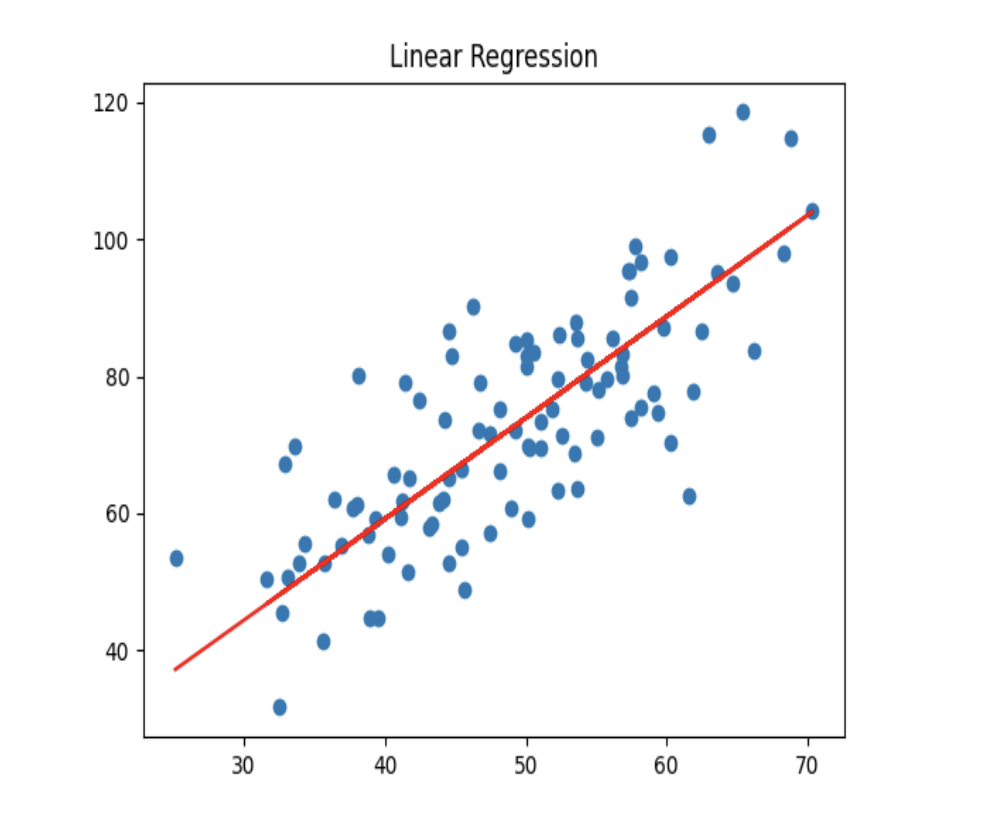
\includegraphics[width=0.64\textwidth]{linear.png}
    %\end{figure}

    \begin{solution}

        Please check the source code and outputs included in the appendix named as

        \begin{center}
            \textbf{CAP\_5610\_Assignment\_2\_Solution\_Arman\_Sayan.ipynb}
        \end{center}
        
        for the solution.
    \end{solution}

    \pagebreak

    \titledquestion{Coding Question}[25]

    Solution for Q5:

    %Please implement a non-linear regression to find the best cubic function model for the 
    %provided non-linear data. Please plot the result, too.

    %\begin{enumerate}[label=(\arabic*)]
    %    \item The cubic function is in the following format: $Y=aX^3+bX^2+cX+d$
    %    \item Use MSE as the loss function.
    %    \item Use Gradient Descent for the training. You may choose fixed learning rate (such as
    %    0.000001 (1e-6)) and epochs (such as 10000) without considering mini-batch. It may take
    %    10-15 seconds to finish the running for 10000 steps. Please be patient.
    %    \item The result will look like the following
    %\end{enumerate}

    %\begin{figure}[h]
    %    \centering
    %    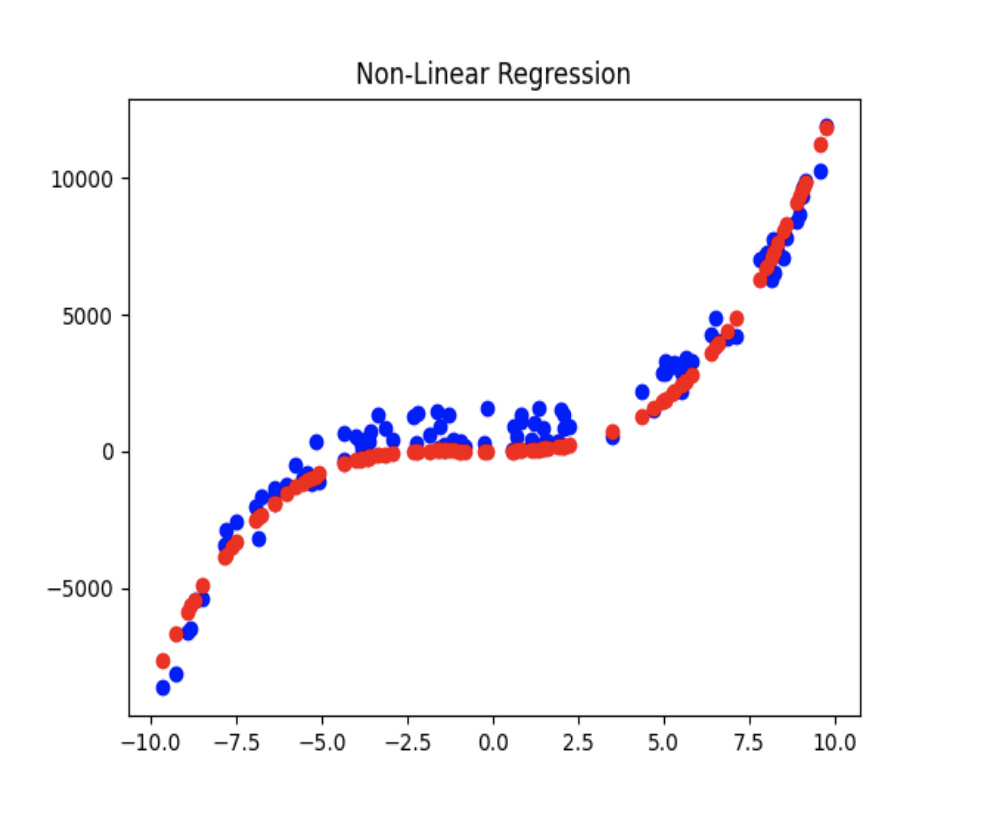
\includegraphics[width=0.65\textwidth]{non-linear.png}
    %\end{figure}

    \begin{solution}

        Please check the source code and outputs included in the appendix named as

        \begin{center}
            \textbf{CAP\_5610\_Assignment\_2\_Solution\_Arman\_Sayan.ipynb}
        \end{center}
        
        for the solution.
    \end{solution}

    \pagebreak
    
\end{questions}

\begin{appendix}
    \centering
    \begin{flushleft}  
      \section{Appendix}
      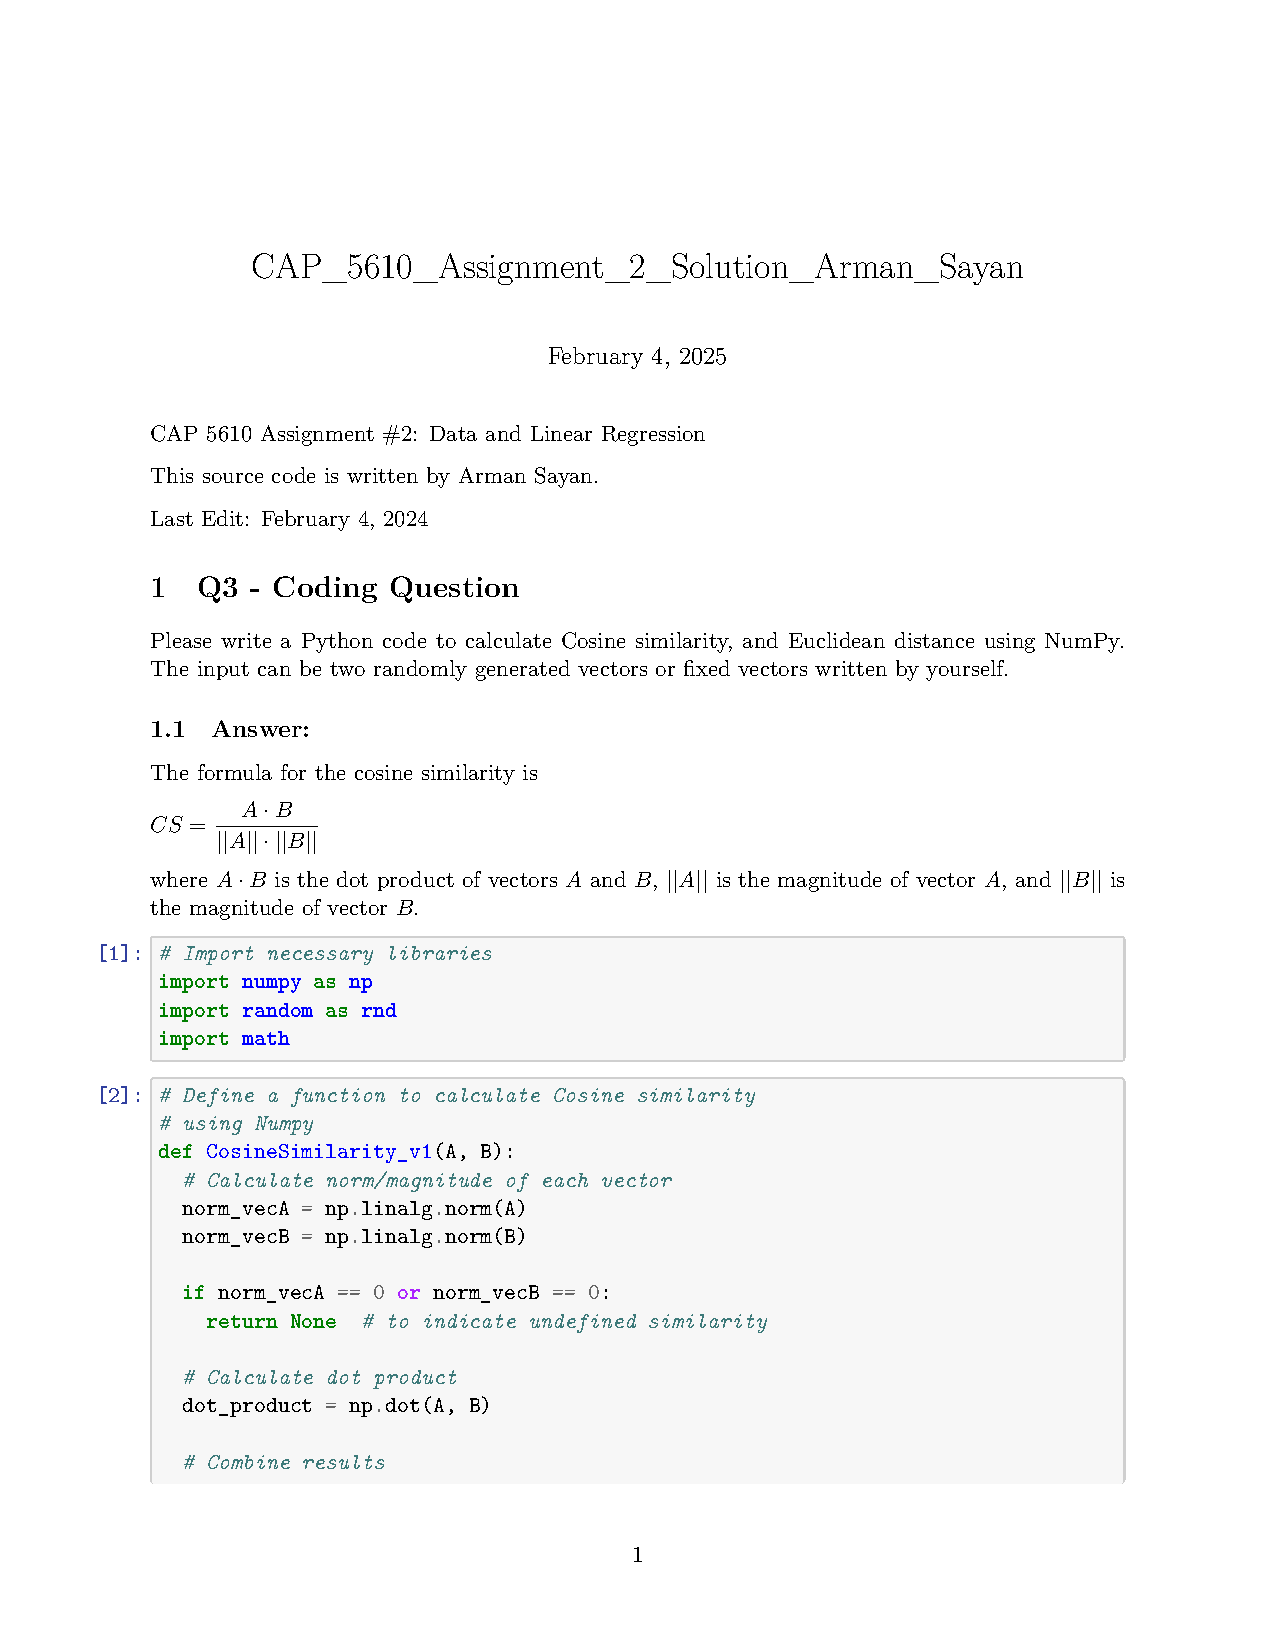
\includepdf[pages=-]{CAP_5610_Assignment_2_Solution_Arman_Sayan_1.pdf}
    \end{flushleft}
\end{appendix}

\end{document}